\documentclass[10pt]{article}
\usepackage[T1]{fontenc}
\usepackage[utf8]{inputenc}
\usepackage{lmodern}
\usepackage[margin=1in]{geometry}
\usepackage{amsmath,amssymb}
\usepackage{booktabs}
\usepackage{array}
\usepackage{xcolor}
\usepackage{listings}
\usepackage{tikz}
\usetikzlibrary{arrows.meta,positioning,shapes.geometric}
\usepackage{pgfplots}
\pgfplotsset{compat=1.16}
\usepackage{enumitem}
\usepackage{url}
\usepackage[hidelinks]{hyperref}

\newcommand{\code}[1]{\texttt{\detokenize{#1}}}
\newcommand{\NaN}{\textsc{NaN}}
\definecolor{codebg}{RGB}{247,247,247}
\definecolor{nanred}{RGB}{214,39,40}
\definecolor{infor}{RGB}{255,127,14}
\definecolor{validblue}{RGB}{31,119,180}
\definecolor{okgreen}{RGB}{44,160,44}
\lstset{basicstyle=\ttfamily\footnotesize, backgroundcolor=\color{codebg}, frame=single, rulecolor=\color{black!20},
        columns=fullflexible, keepspaces=true, breaklines=true, showstringspaces=false,
        keywordstyle=\color{blue!60!black}, commentstyle=\color{green!40!black}, language=Python}

\title{Catching an FP16 Training Divergence with nixnan:\\
From the First Large Value to the First \NaN{} in TinyGPT}
\author{SC26 nixnan tutorial --- \code{flash-attn-expt/fp16-divergence} (branch \code{Flash-Attn})}
\date{October 2026}

\sloppy
\begin{document}
\maketitle

\begin{abstract}
We train TinyGPT, a 4-layer, 0.79M-parameter decoder-only transformer, entirely in IEEE half
precision (FP16). Parameters, activations and gradients are all FP16; there are no FP32 master
weights and no loss scaling. We use plain SGD with momentum at learning rate~1.0, which is high
enough to make training diverge. The run is deterministic: the loss rises from 2.53 to 649 over nine
steps and is \NaN{} at step~10.

We monitor this run with nixnan, an NVBit-based binary instrumentation tool. Without changing the
program, nixnan reports the values crossing $2^9$, $2^{10}$ and $2^{15}$ at the FP16 residual
addition in steps 7, 8 and~9, each attributed to a SASS instruction. In step~10 it reports $\pm\infty$
operands in that addition and then the first \NaN{}, inside LayerNorm's $x-\mu$. A small watcher
kills the run the moment nixnan prints that \NaN{}. An independent PyTorch-side oracle identifies
the same culprit: block~0's attention output projection, whose output reaches $65{,}440$ and then
$\infty$ (FP16's largest finite value is $65{,}504$).

Getting there required four workarounds, and each one says something about the tool. Tile-based
kernels (cuBLAS/CUTLASS GEMMs, flash attention, PyTorch's warp softmax) report false \NaN{}s from
padding lanes in a perfectly healthy first step. \code{MAX_ERRORS} cannot stop at a \NaN{} because
subnormals count too. nixnan's histogram mode crashes on large kernels because of an unbounded
instruction table. And kernel names are truncated. We document each one, with logs.
\end{abstract}

\tableofcontents
\newpage

%=====================================================================================
\section{Goal}

The request was: \emph{make TinyGPT train in FP16 without loss scaling, at a learning rate high
enough to diverge; then catch, with nixnan, the sequence of values that leads to $\infty$ and \NaN{};
stop as soon as the \NaN{} is seen.}

This is the textbook failure mode that mixed-precision training was designed to avoid. Real training
recipes keep FP32 master weights and scale the loss dynamically (\code{torch.cuda.amp.GradScaler}),
and they skip the optimizer step when gradients overflow. We remove all of that on purpose. The
question is whether a binary-level tool, with no knowledge of the model, can show
(1)~\emph{where} the first non-finite value appears, (2)~\emph{how} it propagates, and
(3)~whether the build-up is visible \emph{before} anything overflows.

The short answer is yes on all three, with the caveats of Section~\ref{sec:obstacles}.

%=====================================================================================
\section{Background}

\subsection{FP16}
IEEE binary16 has 1 sign bit, 5 exponent bits and 10 fraction bits. Its largest finite value is
$(2-2^{-10})\cdot 2^{15} = 65{,}504$. Values at or above $65{,}520$ round to $\infty$ in
round-to-nearest. The smallest normal value is $2^{-14}\approx 6.1\times10^{-5}$, and subnormals go
down to $2^{-24}\approx 6\times10^{-8}$. A binade $2^{e}$ means the magnitudes in $[2^{e},2^{e+1})$.
The top binade of FP16 is $2^{15}$, so a value seen in the $2^{15}$ binade is less than a factor of
two from overflow.

\subsection{How PyTorch computes in FP16}
\begin{itemize}[nosep]
\item \textbf{Elementwise kernels} (here \code{CUDAFunctor_add<c10::Half>}) load FP16, convert to
  FP32, compute in FP32 and convert back to FP16 on the store. \code{torch.add(a, b, alpha)} computes
  $a + \alpha b$, which compiles to one \code{FFMA} whose multiplier $\alpha$ is a kernel argument in
  constant bank~0 (\code{c[0x0][0x164]}).
\item \textbf{LayerNorm} (\code{vectorized_layer_norm_kernel<c10::Half, float>}) accumulates the
  row mean and variance in FP32 and normalizes in FP32.
\item \textbf{GEMMs} (\code{nn.Linear} in FP16) run on tensor cores (\code{HMMA.16816.F32}) with
  FP32 accumulation, then round the result to FP16. An accumulated value above $65{,}504$ becomes
  $\pm\infty$ in that final conversion.
\end{itemize}
A consequence that matters for nixnan: in these kernels, most of the FP16 data is \emph{seen as FP32
operands}. The FP16 histogram bins never fire in our run; the FP32 bins do.

\subsection{nixnan}
nixnan is an NVBit tool, loaded with \code{LD_PRELOAD}, that instruments every floating-point SASS
instruction of the kernels it is allowed to touch. It needs no recompilation.
\begin{itemize}[nosep]
\item \textbf{Exceptions mode} (default) checks the operands of each instrumented instruction and
  prints a report when it sees \NaN{}, $\pm\infty$ or a subnormal:
  \begin{lstlisting}[language={}]
#nixnan: error [NaN] detected in operand 0 of instruction FADD R0, R19, -R16 ; in function void at::native:: of type f32
\end{lstlisting}
  Operand~0 is the destination register, so a report on operand~0 means that the instruction
  \emph{produced} the value; operands $1,2,\ldots$ are the sources in SASS order.
\item \textbf{Histogram mode} (\code{HISTOGRAM=1}, \code{BIN_SPEC_FILE}) counts the binades of the
  operands. The bin spec lists exponent ranges per format. A key of the form
  \code{"f32 (record_inst)"} also reports the instruction that caused each threshold hit. With
  \code{"count": 1} and \code{"doublings": N}, a bin reports at its 1st hit, then after 2, 4, 8,
  \ldots{} more, for $N$ doublings, and then resets. This makes the first hit of a bin visible
  without flooding the log.
\item \textbf{Filtering}: \code{FUNCTION_WHITELIST} / \code{FUNCTION_BLACKLIST} take a file of exact
  demangled kernel names. \code{MAX_ERRORS} stops the program after $N$ exception reports.
  \code{LOGFILE} redirects nixnan's output.
\end{itemize}

%=====================================================================================
\section{The experiment}

\subsection{TinyGPT}
TinyGPT (\code{../tinygpt.py}) is the model of the earlier flash-attention study: a pre-LayerNorm
decoder over 12 tokens (digits 0--9, BOS, EOS), with $d_{\text{model}}=128$, 4 heads of dimension~32,
an MLP of width 512 with GELU, rotary position embeddings and no biases. It has 791{,}808
parameters. Each block computes
\[
x \leftarrow x + W_{\text{proj}}\,\mathrm{Attn}(\mathrm{LN}_1(x)),\qquad
x \leftarrow x + W_{\text{fc2}}\,\mathrm{GELU}(W_{\text{fc1}}\,\mathrm{LN}_2(x)).
\]
Attention is PyTorch's SDPA with the flash backend forced. The training set is 100 digit strings, and
the whole set is one batch: 100 sequences of 21 positions.

Two hard-coded \code{.float()} casts in \code{tinygpt.py} were changed to follow the weight dtype, so
the model can run in FP16:
\begin{lstlisting}
x = (idx[..., None] == torch.arange(VOCAB, device=idx.device)).to(self.emb.weight.dtype) @ self.emb.weight
y = flash_attention(q.half(), k.half(), v.half(), causal, self.idx).to(x.dtype)
\end{lstlisting}
The FP32 model is bit-for-bit unchanged: the completion of \code{312} is still \code{312452}.

\subsection{FP16 training without safeguards}
\code{train_fp16.py} (excerpt):
\begin{lstlisting}
model = TinyGPT().cuda().half()                    # FP16 everything, no master weights
opt = torch.optim.SGD(model.parameters(), lr=a.lr, momentum=0.9)
for step in range(1, a.steps + 1):
    logits = model(x)
    loss = F.cross_entropy(logits.reshape(-1, logits.shape[-1]).float(), y.reshape(-1), ignore_index=-100)
    opt.zero_grad(set_to_none=True)
    loss.backward()
    lv = loss.item()
    print(f"step {step:4d}  loss {lv:.4f}", flush=True)
    if lv != lv or abs(lv) == float("inf"):
        print(f"STOP: non-finite loss at step {step}", flush=True)
        break
    opt.step()
\end{lstlisting}
The only FP32 computation is the cross-entropy on the logits, which are cast to FP32 so that the loss
value itself is meaningful. There is no \code{GradScaler}, no gradient clipping and no master copy;
\code{opt.step()} updates the FP16 parameters in place.

\paragraph{Why SGD at lr 1.0.} SGD's update is $\Delta w = -\eta\,(\text{momentum-averaged
gradient})$, so the step size grows with the gradient and the weights can grow without bound. (AdamW,
used in \code{../train.py}, normalizes the update and would diverge far more slowly.) At $\eta=1$
TinyGPT diverges in ten steps, which keeps the nixnan runs short.

\paragraph{Determinism.} The seed is fixed and the whole data set is one batch. Every run we made,
with or without nixnan, printed the same loss sequence to four decimals.

\subsection{The oracle}
\code{train_fp16.py --oracle} registers a forward hook on every leaf module and, after each
backward pass, prints the largest finite $|\cdot|$ over activations, gradients and parameters, the
tensor that holds the largest value, and the first tensor (in forward order, then gradients, then
parameters) that contains a non-finite value. The oracle launches its own kernels, so it is never run
under nixnan. It is the ground truth that nixnan's reports are checked against.

%=====================================================================================
\section{What the oracle sees}

Table~\ref{tab:oracle} is \code{logs/oracle-lr1.txt}. Figure~\ref{fig:climb} plots it.

\begin{table}[h]
\centering\small
\begin{tabular}{rrrrrl}
\toprule
step & loss & max $|$act$|$ & max $|$grad$|$ & max $|$param$|$ & largest activation \\
\midrule
1 & 2.5254 & 4.77 & 0.147 & 1.00 & \code{blocks.1.ln2} \\
2 & 2.4189 & 4.66 & 0.109 & 1.005 & \code{blocks.2.ln2} \\
3 & 3.1881 & 9.85 & 0.622 & 1.011 & \code{head} \\
4 & 24.8335 & 24.3 & 2.23 & 1.015 & \code{head} \\
5 & 6.7435 & 47.6 & 0.821 & 1.52 & \code{head} \\
6 & 79.3333 & 87.0 & 6.27 & 3.23 & \code{head} \\
7 & 169.8536 & 815.5 & 25.8 & 6.47 & \code{blocks.0.proj} \\
8 & 198.7644 & 1{,}315 & 29.4 & 23.7 & \code{blocks.0.proj} \\
9 & 649.3550 & 29{,}570 & 41.3 & 46.3 & \code{blocks.0.proj} \\
10 & \textcolor{nanred}{\NaN} & 65{,}440 + \textcolor{infor}{7{,}870 $\infty$} & \textcolor{nanred}{\NaN} & 66.1 & \code{blocks.0.proj} \\
\bottomrule
\end{tabular}
\caption{Oracle, one row per training step (values after the forward and backward pass of that
step). At step 10 the first non-finite tensor is the \emph{output of} \code{blocks.0.proj}: 7{,}870
$\infty$ and no \NaN{}.}
\label{tab:oracle}
\end{table}

\begin{figure}[h]
\centering
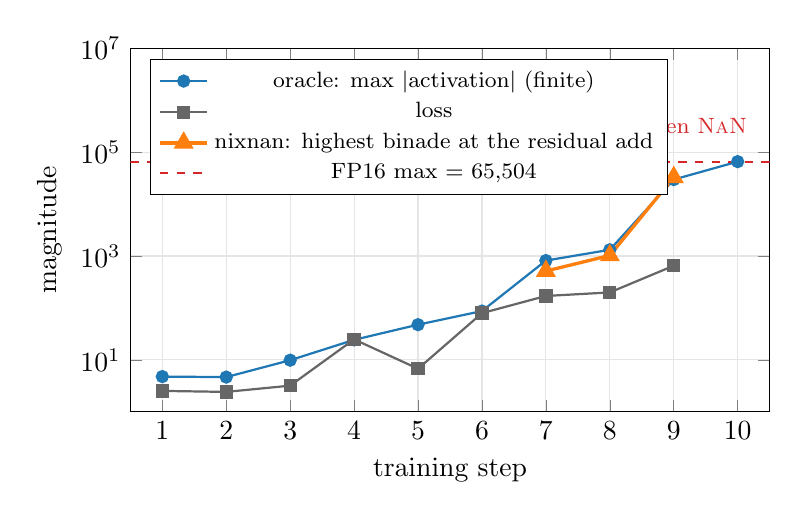
\begin{tikzpicture}
\begin{semilogyaxis}[width=0.8\textwidth, height=6.2cm, xlabel={training step}, ylabel={magnitude},
  xmin=0.5, xmax=10.5, ymin=1, ymax=1e7, xtick={1,...,10}, legend pos=north west,
  legend style={font=\footnotesize}, grid=major, grid style={black!10}]
\addplot[validblue, thick, mark=*] coordinates {(1,4.766)(2,4.66)(3,9.852)(4,24.31)(5,47.59)(6,87)(7,815.5)(8,1315)(9,29570)(10,65440)};
\addlegendentry{oracle: max $|$activation$|$ (finite)}
\addplot[black!60, thick, mark=square*] coordinates {(1,2.5254)(2,2.4189)(3,3.1881)(4,24.8335)(5,6.7435)(6,79.3333)(7,169.8536)(8,198.7644)(9,649.355)};
\addlegendentry{loss}
\addplot[infor, very thick, mark=triangle*, mark size=3pt] coordinates {(7,512)(8,1024)(9,32768)};
\addlegendentry{nixnan: highest binade at the residual add}
\addplot[nanred, dashed, thick, domain=0.5:10.5] {65504};
\addlegendentry{FP16 max = 65{,}504}
\node[nanred, font=\footnotesize, anchor=south east] at (axis cs:10.3,1.2e5) {step 10: $\infty$, then \NaN};
\end{semilogyaxis}
\end{tikzpicture}
\caption{The climb. nixnan's histogram (orange; lower edge of the binade) tracks the oracle's
activation maximum from step 7 on, three steps before the overflow.}
\label{fig:climb}
\end{figure}

What happens:
\begin{enumerate}[nosep]
\item Steps 1--6: the weights grow (max $|w|$ goes from 1.0 to 3.2), and the logits (\code{head})
  hold the largest activations. The loss oscillates and climbs.
\item Step 7: block~0's attention output projection takes over. Its output grows by a factor
  $\approx 1.6$, then $\approx 22$, then $\approx 2.2$ per step: its weights grow (max $|w|$ reaches 46 at
  step 9) and so does its input, and the two multiply.
\item Step 10: the projection's FP32-accumulated outputs exceed $65{,}504$ for 7{,}870 elements.
  They round to $\pm\infty$ when the GEMM writes FP16. The other elements stay finite (the largest is
  $65{,}440$, two FP16 ulps of 32 below the maximum). The \NaN{} in the loss comes from what
  happens next.
\end{enumerate}

%=====================================================================================
\section{The nixnan setup}

The final setup is \code{run_nixnan.sh}; Section~\ref{sec:obstacles} explains why it looks the way it
does.

\begin{lstlisting}[language=bash]
# pass 0: log every kernel name (dummy whitelist -> nothing is instrumented)
env LD_PRELOAD=$NN FUNCTION_WHITELIST=logs/dummy-whitelist.txt LOGFILE=logs/kernels-names.log \
    python train_fp16.py --lr 1
names | grep -E "pytorch_flash|cutlass|^ampere_|cublasLt|softmax_warp" > blacklist.txt
names | grep -E "CUDAFunctor_add<c10::Half>|vectorized_layer_norm_kernel<c10::Half" > hist-whitelist.txt

# pass 1: exceptions in every other kernel, killed at the first NaN report
python3 watch_nan.py logs/nixnan-exceptions.log -- \
    env LD_PRELOAD=$NN FUNCTION_BLACKLIST=blacklist.txt python train_fp16.py --lr 1

# pass 2: binade histogram with instruction attribution, two kernels, same watcher
python3 watch_nan.py logs/nixnan-climb.log -- \
    env LD_PRELOAD=$NN FUNCTION_WHITELIST=hist-whitelist.txt BIN_SPEC_FILE=spec-climb.json HISTOGRAM=1 \
    python train_fp16.py --lr 1
python3 summarize_climb.py logs/nixnan-climb.log logs/nixnan-exceptions.log > logs/SUMMARY.txt
\end{lstlisting}

\paragraph{Pass 0 (kernel names).} One training run uses 50 distinct kernels. nixnan prints each
kernel's full demangled name when it launches, even when nothing is instrumented. Whitelists and
blacklists need exactly these names, so they are generated rather than written by hand.

\paragraph{Pass 1 (exceptions).} 18 kernels are blacklisted (Table~\ref{tab:blacklist}). All of them
are tile-based and compute on lanes outside the tensor (Section~\ref{sec:fp}). Every other kernel
is checked for \NaN{}, $\pm\infty$ and subnormals.

\begin{table}[h]
\centering\small
\begin{tabular}{>{\raggedright\arraybackslash}p{6.6cm}r>{\raggedright\arraybackslash}p{6.2cm}}
\toprule
family & kernels & why \\
\midrule
cuBLAS \code{ampere_fp16_s16816gemm_*}, \code{s1688gemm_*} & 4 & GEMM tiles \\
\code{cutlass::Kernel2<cutlass_80_*gemm*>} & 6 & GEMM tiles (\NaN{} at step 1, \code{logs/false-positive-gemm-step1.log}) \\
\code{cublasLt::splitKreduce_kernel} & 2 & split-K reduction of a GEMM \\
\code{pytorch_flash::flash_*} (fwd, bwd, \code{dot_do_o}, \code{convert_dq}) & 4 & padding lanes (\code{../PyTorch_Instrumentation/PyT.md}) \\
\code{softmax_warp_forward/backward} & 2 & $-\infty$ padding (\code{logs/false-positive-}\newline\code{softmax-step1.log}) \\
\bottomrule
\end{tabular}
\caption{\code{blacklist.txt}, generated in pass 0.}
\label{tab:blacklist}
\end{table}

Blacklisting the GEMMs does not hide a GEMM overflow. An $\infty$ written by a GEMM is read by the
next kernel, and nixnan sees it there as an $\infty$ source operand. That is exactly how the step-10
overflow shows up.

\paragraph{Pass 2 (histogram).} \code{spec-climb.json}:
\begin{lstlisting}[language={}]
{ "count": 1, "doublings": 20,
  "f16 (record_inst)": [[9,9],[10,10],[11,11],[12,12],[13,13],[14,14],[15,15]],
  "f32 (record_inst)": [[9,9],[10,10],[11,11],[12,12],[13,13],[14,14],[15,15],[16,17]],
  "bf16": [], "f64": [] }
\end{lstlisting}
One bin per binade from $2^9$ ($\geq 512$) to $2^{15}$ (the top FP16 binade), for FP16 and FP32
operands, plus one FP32 bin for $2^{16}$--$2^{17}$ (values FP16 cannot hold). Each bin reports its
first hit, with the instruction. The whitelist holds the two kernels that touch the residual stream
in FP16: the residual addition and LayerNorm. The histogram cannot cover every kernel
(Section~\ref{sec:crash}).

\paragraph{The watcher.} \code{watch_nan.py} runs the command, prefixes every output line with the
elapsed time, and on the first line that matches \verb|#nixnan: error \[[^\]]*NaN| writes a
\code{WATCHER} line and kills the whole process group with \code{SIGKILL}. Subnormal and $\pm\infty$
reports do not stop it.

\paragraph{Reading the log by step.} \code{train_fp16.py} prints \code{step N loss X} after the
backward pass of step $N$. Everything nixnan prints after the line for step $N-1$ therefore belongs to
step $N$'s forward and backward pass. \code{summarize_climb.py} uses this to group the reports by
step and keeps, per kernel and format, the highest binade reached and the instructions that reached
it.

%=====================================================================================
\section{Results}

\subsection{The timeline}

Table~\ref{tab:timeline} condenses \code{logs/SUMMARY.txt}.

\begin{table}[h]
\centering\small
\begin{tabular}{rr>{\raggedright\arraybackslash}p{3.7cm}>{\raggedright\arraybackslash}p{3.5cm}>{\raggedright\arraybackslash}p{4.3cm}}
\toprule
step & loss & residual add (\code{CUDAFunctor_add}), FP32 operands & LayerNorm, FP32 operands & exception reports \\
\midrule
1--3 & 2.53--3.19 & below $2^9$ & below $2^9$ & none \\
4 & 24.8 & below $2^9$ & $2^{10}$ (\code{FADD}, \code{FFMA}) & none \\
5 & 6.74 & below $2^9$ & $2^{13}$ & none \\
6 & 79.3 & below $2^9$ & $2^{17}$ (\code{FMUL}: sums of squares) & none \\
7 & 169.9 & \textbf{$2^9$} ($\geq 512$), \code{FFMA}; 3{,}040 reports & $2^{17}$ & none (subnormals only) \\
8 & 198.8 & \textbf{$2^{10}$} ($\geq 1{,}024$); 1{,}292 reports & $2^{17}$ (+\code{MUFU.RSQ}) & none \\
9 & 649.4 & \textbf{$2^{15}$} ($\geq 32{,}768$); 49{,}144 reports & $2^{17}$; 168{,}254 reports & none \\
10 & --- & $2^{15}$, then \textcolor{infor}{$\pm\infty$} & \textcolor{infor}{$-\infty$}, then \textcolor{nanred}{\NaN} & add: $\pm\infty$ in \code{FFMA}; LayerNorm: $-\infty$, then \textbf{\NaN{}} $\Rightarrow$ \textbf{killed} \\
\bottomrule
\end{tabular}
\caption{Per-step timeline from the histogram pass (columns 3--4) and both passes (column 5).
``$2^e$'' is the highest binade any instrumented instruction saw.}
\label{tab:timeline}
\end{table}

\paragraph{The residual add is the early warning.} Its operands are the residual stream $x$ and the
block outputs. They cross 512 in step 7, 1{,}024 in step 8 and 32{,}768 in step 9, less than a factor
of two from FP16's maximum. Every report names the instruction, always the same one:
\code{FFMA Rd, Ra, c[0x0][0x164], Rc}, i.e.\ $d = \alpha\,b + a$. The oracle's maxima (815, 1{,}315,
29{,}570) fall in exactly these binades.

\paragraph{LayerNorm's large FP32 values are harmless.} From step 4 on, LayerNorm's FP32 bins fire,
and from step 6 they reach $2^{17}$, a range FP16 cannot represent. These are the FP32 accumulations
of $\sum (x-\mu)^2$ for the variance (\code{FMUL}, \code{FFMA}) and \code{MUFU.RSQ} of the variance.
They are FP32 and never stored as FP16. A user reading the histogram must tell them apart from the
residual stream, which is why the add is the useful signal.

\paragraph{The FP16 bins never fire.} Both kernels convert to FP32 before computing (Section 2.2), so
nixnan classifies every arithmetic operand as FP32. A bin spec with only \code{f16} keys would show
nothing.

\subsection{Step 10, report by report}
\label{sec:step10}

The histogram pass printed these exception reports in step 10, in this order (bin reports omitted):

\begin{lstlisting}[language={}]
[54.0s] error [-infinity] operand 1 of FFMA R6, R7, c[0x0][0x164], R6   ; vectorized_elementwise_kernel (add)
[54.0s] error [-infinity] operand 0 of FFMA R6, R7, c[0x0][0x164], R6
[54.0s] error [infinity]  operand 1 of FFMA R9, R9, c[0x0][0x164], R8
[54.0s] error [infinity]  operand 0 of FFMA R9, R9, c[0x0][0x164], R8
[54.0s] error [infinity]  operand 1 of FFMA R10, R11, c[0x0][0x164], R10
[54.0s] error [infinity]  operand 0 of FFMA R10, R11, c[0x0][0x164], R10
[54.0s] error [-infinity] operand 1 of FADD R18, R19, -R16                ; void at::native:: (LayerNorm)
[54.0s] error [-infinity] operand 0 of FADD R18, R19, -R16
[54.0s] error [-infinity] operand 1 of FFMA R16, R18, R15, R16
[54.0s] error [-infinity] operand 0 of FFMA R16, R18, R15, R16
[54.0s] error [-infinity] operand 1 of FADD R0, R19, -R16
[54.0s] error [-infinity] operand 2 of FADD R0, R19, -R16
[54.0s] error [NaN]       operand 0 of FADD R0, R19, -R16
[54.0s] WATCHER: first nixnan NaN report -- killing the run
\end{lstlisting}

\begin{figure}[h]
\centering
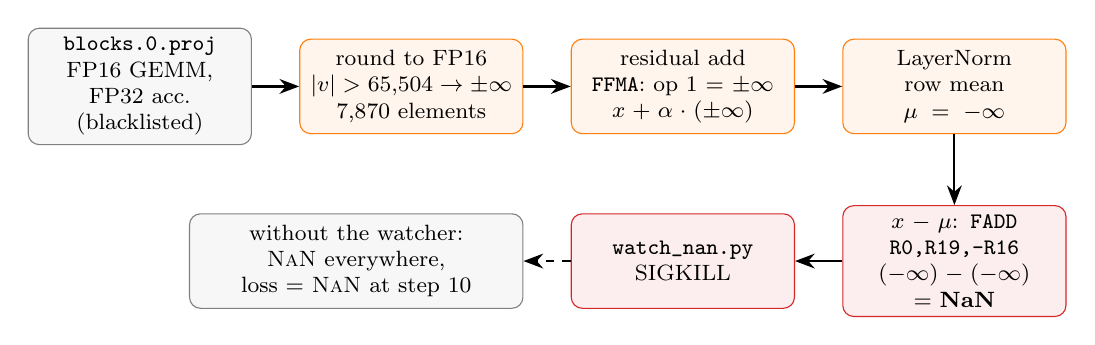
\begin{tikzpicture}[node distance=6mm, every node/.style={font=\footnotesize, align=center},
  box/.style={draw, rounded corners, minimum height=12mm, text width=26mm, fill=black!3},
  arr/.style={-{Stealth[length=2.5mm]}, thick}]
\node[box, draw=black!50] (g) {\code{blocks.0.proj}\\ FP16 GEMM, FP32 acc.\\ (blacklisted)};
\node[box, right=of g, draw=infor, fill=infor!8] (r) {round to FP16\\ $|v|>65{,}504\to\pm\infty$\\ 7{,}870 elements};
\node[box, right=of r, draw=infor, fill=infor!8] (a) {residual add\\ \code{FFMA}: op 1 $=\pm\infty$\\ $x+\alpha\cdot(\pm\infty)$};
\node[box, right=of a, draw=infor, fill=infor!8] (m) {LayerNorm\\ row mean\\ $\mu=-\infty$};
\node[box, below=9mm of m, draw=nanred, fill=nanred!8] (n) {$x-\mu$: \code{FADD R0,R19,-R16}\\ $(-\infty)-(-\infty)$\\ $=$ \textbf{\NaN}};
\node[box, left=of n, draw=nanred, fill=nanred!8] (k) {\code{watch_nan.py}\\ SIGKILL};
\node[box, left=of k, draw=black!50, text width=40mm] (o) {without the watcher: \NaN{} everywhere,\\ loss $=$ \NaN{} at step 10};
\draw[arr] (g) -- (r); \draw[arr] (r) -- (a); \draw[arr] (a) -- (m); \draw[arr] (m) -- (n);
\draw[arr] (n) -- (k); \draw[arr, dashed] (k) -- (o);
\end{tikzpicture}
\caption{How the step-10 overflow becomes a \NaN{}. Orange: $\pm\infty$; red: \NaN.}
\label{fig:chain}
\end{figure}

Decoding them, with Figure~\ref{fig:chain}:
\begin{enumerate}
\item \textbf{The residual add receives $\pm\infty$.} In \code{FFMA R9, R9, c[0x0][0x164], R8}, the
  sources are $R9 = b$ (the \code{other} tensor of \code{torch.add}), the constant $\alpha$ and
  $R8 = a$. For \code{x + self.proj(y)}, $b$ is the projection's output. Operand~1 ($b$) is $\infty$,
  and so is operand~0 (the sum written back). The add did not create the $\infty$; it read it. Since
  the GEMMs are blacklisted, this is the first instrumented instruction to see the overflow, and the
  oracle confirms that the producer is \code{blocks.0.proj}.
\item \textbf{LayerNorm's mean becomes $-\infty$.} The next kernel to read the residual stream is
  block~0's \code{ln2}. \code{FADD R18, R19, -R16} followed by \code{FFMA R16, R18, R15, R16} has the
  shape of a running-mean update ($\delta = x-\mu$; $\mu \mathrel{+}= \delta\cdot\tfrac1n$), and the
  reports show an element $x=-\infty$ making $\delta$ and then $\mu$ equal to $-\infty$.
\item \textbf{The first \NaN{}.} \code{FADD R0, R19, -R16} computes $x-\mu$ with $x$ (operand 1) and
  $\mu$ (operand 2) both $-\infty$. The result (operand 0) is $(-\infty)-(-\infty)=\NaN$. This is the
  birth of the \NaN{}, and the watcher kills the run in the same second.
\end{enumerate}
Had the run continued, the \NaN{} would have entered the variance, the normalized row, every
following layer, the logits and the loss: the oracle's run shows loss $=\NaN$ and \NaN{} gradients at
step~10.

\subsection{The exceptions pass agrees}
Pass~1 instruments 32 kernels (all but the 18 blacklisted). It runs for 213~s and prints:
\begin{itemize}[nosep]
\item no exception report in steps 1--7;
\item 18 subnormal reports from step 8 on, in GELU's \code{FMUL}s (\code{0.3989\ldots} $=1/\sqrt{2\pi}$);
\item in step 10, the same six $\pm\infty$ reports in the add's three \code{FFMA}s, the same
  $-\infty$ reports in LayerNorm, and then the first \NaN{}, killed.
\end{itemize}
In this pass the first \NaN{} report is \code{operand 2 of FFMA R17, R18, R0, R17}, the instruction
that consumes $R0 = x-\mu$, instead of the \code{FADD} that produced it. Both are in the same kernel,
step and row computation. Which one prints first depends on which warp's report reaches nixnan's
channel first; in our runs both orders occurred. It is always LayerNorm in step~10.

\subsection{Reproducibility}
We reran \code{run_nixnan.sh} from scratch (5~min 20~s). The loss sequence, the histogram timeline
and the step-10 \code{FFMA}/\code{FADD} sequence were identical. The only difference was the
first-\NaN{} instruction described above.

%=====================================================================================
\section{Obstacles, and what they say about nixnan}
\label{sec:obstacles}

\subsection{False \NaN{}s in a healthy first step}
\label{sec:fp}
Our first attempt instrumented every kernel and used the watcher. It stopped at \emph{step~1}, while
the oracle shows every tensor of step~1 finite and bounded by~5.

\paragraph{CUTLASS GEMM.} \code{logs/false-positive-gemm-step1.log}, 94~s into the run:
\begin{lstlisting}[language={}]
#nixnan: error [NaN,subnormal] detected in operand 1 of instruction HMMA.16816.F32 R20, R48.reuse, R46, R20 ; in function void cutlass::Kernel2 of type f16
\end{lstlisting}
A GEMM tile loads its A and B fragments from shared memory. When the problem does not fill the tile
(for instance the 12-row vocabulary projection, far smaller than a tile), the
out-of-range lanes compute on whatever bits are there, and only the in-range results are stored.
The \NaN{} is real in the register but never reaches a tensor.

\paragraph{Warp softmax.} With GEMMs blacklisted, the next stop was
\code{softmax_warp_forward} in \code{cross_entropy} (\code{logs/false-positive-softmax-step1.log}):
\begin{lstlisting}[language={}]
#nixnan: error [-infinity] detected in operand 0 of instruction FFMA R8, R7, 1.4426950216293334961, -R8 ; in function void  of type f32
#nixnan: error [NaN] detected in operand 0 of instruction FADD R7, -R12, R7 ; in function void  of type f32
\end{lstlisting}
PyTorch's warp softmax loads out-of-range elements as $-\infty$, so each warp can process whole
rows of a power-of-two width. In a valid row, the padding elements give
$(-\infty-\max)\cdot\log_2 e=-\infty$ (the first report; \code{1.4426\ldots} $=\log_2 e$) and
$\exp(-\infty)=0$, which is harmless. In a row slot past the last row, every element is $-\infty$,
so $\max=-\infty$ and $x-\max=(-\infty)-(-\infty)=\NaN$ (the second report). Such rows are never
stored.

\paragraph{Same as flash.} This is the padding-lane effect we documented for flash attention
(\code{../PyTorch_Instrumentation/PyT.md}). For a tool that checks register operands, any
tile-based kernel can report \NaN{}s that are not in the program's data. Blacklisting these kernels is
the practical answer, and it costs nothing here because their outputs are checked by the next kernel.
A future nixnan could check stores (\code{INSTR_MEM}) instead of arithmetic for such kernels, or
let users blacklist by pattern rather than exact name.

\subsection{\code{MAX\_ERRORS} cannot stop at a NaN}
\code{MAX_ERRORS=1} stops after the first exception report of any kind, and subnormals count. With
GEMMs instrumented, FP16 training reports subnormal \code{HMMA} operands at step~1 (34~s in), long
before any overflow. Even with GEMMs blacklisted, GELU's subnormals come at step~8, two steps before
the \NaN{}. We need ``stop at the first \NaN{}'', which nixnan does not offer, so \code{watch_nan.py}
supplies it from outside. A \code{MAX_NANS} (or a category mask for \code{MAX_ERRORS}) would make it
unnecessary.

\subsection{The histogram crashes on large kernels}
\label{sec:crash}
With \code{HISTOGRAM=1} and no whitelist, the run segfaults (\code{logs/histogram-crash.log}
ends abruptly at 39~s). Under gdb:
\begin{lstlisting}[language={}]
Thread 1 "python" received signal SIGSEGV, Segmentation fault.
... std::__cxx11::basic_string<...>::_M_assign(...)
#3  nixnan::recorder::mk_entry (this=..., instr="FFMA R12, R10, R2.reuse, R13 ;", path="", line="0",
      func="void cutlass::Kernel2", ...)
\end{lstlisting}
\code{recorder::mk_entry} (\code{src/recording.cu:88}) is:
\begin{lstlisting}[language=C++]
inst_info[current_entry].instr = instr;
inst_info[current_entry].path  = path;
...
return current_entry++;
\end{lstlisting}
with \code{inst_info} allocated for \code{TABLE_SIZE} $=2^{17}$ entries (\code{src/nixnan.cu:71}) and
no bounds check. With \code{record_inst} keys, every FP instruction of every instrumented kernel gets
an entry. The large GEMM kernels push \code{current_entry} past the end, the string assignments write
into freed or foreign heap memory, and the process dies. We did not modify nixnan; restricting the
histogram to two kernels keeps the table small. The fix is a bounds check (or a growable table), plus
deduplication of entries per (function, offset).

\subsection{Truncated kernel names}
nixnan's \code{cut_kernel_name} keeps the demangled name up to the first \code{<} or \code{(}:
\begin{lstlisting}[language=C++]
size_t pos = kernel_name.find_first_of("<(");
\end{lstlisting}
So \code{void at::native::(anonymous namespace)::vectorized_layer_norm_kernel<c10::Half, float>(...)}
prints as \code{void at::native::}, and the warp softmax prints as \code{void }. Every elementwise
kernel prints as \code{void at::native::vectorized_elementwise_kernel}. In the exception reports,
LayerNorm is identifiable only because the histogram pass instruments just two kernels (the bin
reports, which come from another code path, carry the full name). Cutting at the template list
\emph{after} the function name, or printing the full name once per kernel with a short id, would fix
this.

%=====================================================================================
\section{Discussion}

\paragraph{What nixnan showed that the loss curve does not.}
The loss curve says the run is unstable from step 4 and dead at step 10. nixnan says, without source
changes: which instruction in which kernel first saw an $\infty$ (the residual add's \code{FFMA},
operand 1, i.e.\ an overflowed GEMM output), which instruction first produced a \NaN{}
(LayerNorm's $x-\mu$), the arithmetic reason ($-\infty-(-\infty)$), and three steps of warning in
which the residual stream climbs binade by binade towards $65{,}504$.

\paragraph{What it took.}
It took a model of the program to aim the tool: which kernels are tile-based (blacklist), which
kernels carry the residual stream (histogram whitelist), and that FP16 data is computed on as FP32
(bin spec). It took a watcher for ``stop at the first \NaN{}''. And the oracle was needed to name the
blacklisted producer (\code{blocks.0.proj}), which nixnan can only see indirectly.

\paragraph{What a fix would look like.}
For the training run itself, the standard fixes each address one link of Figure~\ref{fig:chain}: a
smaller learning rate or AdamW (no growth), gradient clipping, FP32 master weights with
\code{GradScaler} (overflow detected and the step skipped), or BF16 (8 exponent bits: the same values
would be finite). nixnan's histogram would show the first two as a residual stream that never
climbs.

%=====================================================================================
\section{Files and reproduction}

All under \code{flash-attn-expt/fp16-divergence/}:

\begin{center}\small
\begin{tabular}{>{\raggedright\arraybackslash}p{4.6cm}p{10cm}}
\toprule
\code{train_fp16.py} & FP16 training; stops at the first non-finite loss; \code{--oracle} \\
\code{watch_nan.py} & runs a command, timestamps its output, kills it at the first nixnan \NaN{} report \\
\code{run_nixnan.sh} & passes 0--2, summary, oracle ($\approx$5 min on an RTX 3090) \\
\code{blacklist.txt}, \code{hist-whitelist.txt},\newline \code{spec-climb.json} & nixnan configuration \\
\code{summarize_climb.py} & per-step timeline from the logs \\
\code{logs/SUMMARY.txt} & the timeline (Table~\ref{tab:timeline}) \\
\code{logs/nixnan-exceptions.log} & pass 1 \\
\code{logs/nixnan-climb.log.xz} & pass 2 (398k lines) \\
\code{logs/oracle-lr1.txt} & Table~\ref{tab:oracle} \\
\code{logs/false-positive-}\newline\code{*-step1.log} & Section~\ref{sec:fp} \\
\code{logs/histogram-crash.log} & Section~\ref{sec:crash} \\
\code{logs/kernels-names.log} & pass 0 \\
\code{latex/} & this report and the slides \\
\bottomrule
\end{tabular}
\end{center}

Environment: PyTorch 2.6.0+cu124 (venv \code{~/repos/newmed/venv}), CUDA 12.4, RTX 3090 (sm\_86),
nixnan from \code{external/nixnan} (NVBit 1.8), unmodified.

\end{document}
